Two circuits are given in Figures \ref{fig:example1} and \ref{fig:example2},
by circuit diagrams and by the language defined above. 

\begin{figure}[htbp]
  \begin{subfigure}{\textwidth}
    \centering
    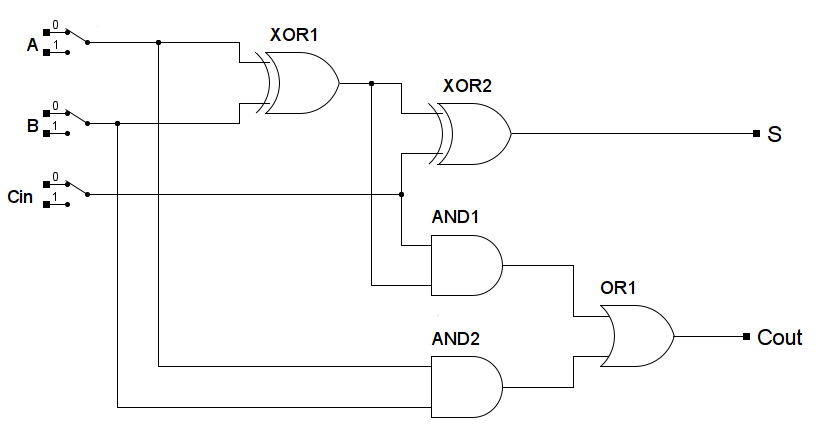
\includegraphics[scale=.33]{examples/fulladder.png}
    \caption{Circuit diagram for a full adder}
  \end{subfigure}
  \begin{subfigure}{\textwidth}
    \lstinputlisting{examples/fulladder.circuit}
    \caption{Full adder described by our language}
  \end{subfigure}
  \caption{A full adder, described equivalently by a standard circuit
    diagram and by our language.}
  \label{fig:example1}
\end{figure}

% make p figure align to top of page, as per request by ff300
\begingroup
\makeatletter
\setlength{\@fptop}{0pt}
\setlength{\@fpbot}{0pt plus 1fil}
\makeatother
\begin{figure}[p]
  \begin{subfigure}{\textwidth}
    \centering
    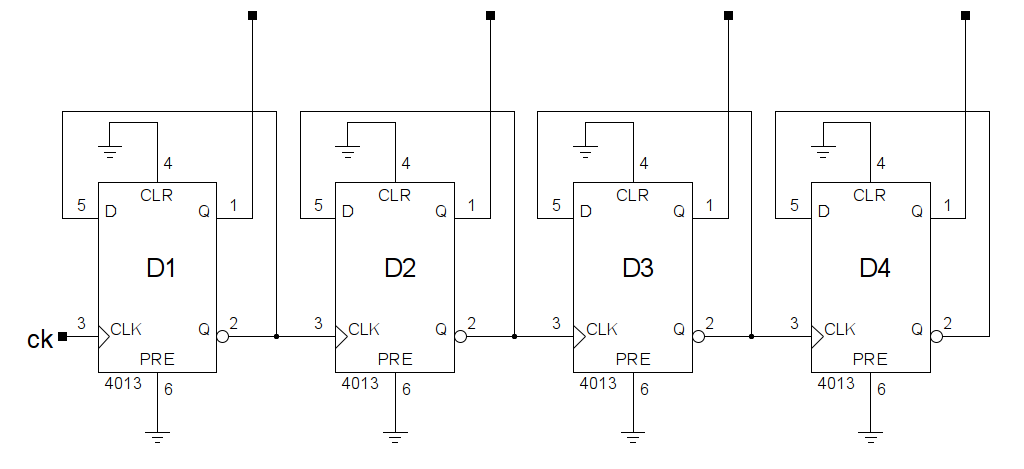
\includegraphics[scale=.33]{examples/ripplecounter.png}
    \caption{Circuit diagram for a ripple counter}
  \end{subfigure}
  \begin{subfigure}{\textwidth}
    \lstinputlisting{examples/ripplecounter.circuit}
    \caption{Ripple counter described by our language}
  \end{subfigure}
  \caption{A 4-bit ripple counter. Note that the circuit diagram is
    slightly simplified by implementing \texttt{gnd} directly as
    ground instead of a switch set to \texttt{0}, to avoid clutter
    in the diagram.}
  \label{fig:example2}
\end{figure}
\clearpage % outputs all floats
\endgroup
